%  ========================================================================
%  Copyright (c) 2006-2008 The University of Washington
%
%  Licensed under the Apache License, Version 2.0 (the "License");
%  you may not use this file except in compliance with the License.
%  You may obtain a copy of the License at
%
%      http://www.apache.org/licenses/LICENSE-2.0
%
%  Unless required by applicable law or agreed to in writing, software
%  distributed under the License is distributed on an "AS IS" BASIS,
%  WITHOUT WARRANTIES OR CONDITIONS OF ANY KIND, either express or implied.
%  See the License for the specific language governing permissions and
%  limitations under the License.
%  ========================================================================
%

% Documentation for UW thesis document style for LaTeX
% by Jim Fox
% fox@washington.edu
%
%    Revised for version 2008/04/15 of uwthesis.cls
%
%    This document is contained in a single file ONLY because
%    I wanted to be able to distribute it easily.  A real thesis ought
%    to be contained on many files (e.g., one for each chapter, at least).
%
%    To help you identify the files and sections in this large file
%    I use the string '==========' to identify new files.
%
%    To help you ignore the unusual things I do with this sample document
%    I try to use the notation
%       
%    % --- sample stuff only -----
%    special stuff for my document, but you don't need it in your thesis
%    % --- end-of-sample-stuff ---


%    Printed in twoside style now that that's allowed
%
 
\documentclass [11pt, twoside] {uwthesis}
 
%
% The following line would print the thesis in a postscript font 

% \usepackage{newcent}

\setcounter{tocdepth}{1}  % Print the chapter and sections to the toc
 

% ==========   Local defs and mods
%

% --- sample stuff only -----
% These format the sample code in this document

\usepackage{alltt}  % 
\newenvironment{demo}
  {\begin{alltt}\leftskip3em
     \def\\{\ttfamily\char`\\}%
     \def\{{\ttfamily\char`\{}%
     \def\}{\ttfamily\char`\}}}
  {\end{alltt}}
 
% metafont font.  If logo not available, use the second form
%
% \font\mffont=logosl10 scaled\magstep1
\let\mffont=\sf
% --- end-of-sample-stuff ---
 



\begin{document}
 
% ==========   Preliminary pages
%

\prelimpages
 
%
% ----- title page
%
\Title{The Suitability of the \LaTeX\ Text Formatter\\
  for Thesis Preparation by Technical and\\
  Non-technical Degree Candidates}
\Author{Jim Fox}
\Year{2008}
\Program{UW Technology Services}
% \titlepage  

% --- sample stuff only -----
% unusual footnote not found in a real thesis
{\Degreetext{A dissertation%
  \footnote[2]{an egocentric imitation, actually}
  submitted in partial fulfillment of\\
  the requirements for the degree of}
 \def\thefootnote{\fnsymbol{footnote}}
 \let\footnoterule\relax
 \titlepage
 }
\setcounter{footnote}{0}
% --- end-of-sample-stuff ---
 
%
% ----- signature page (put real names in these)
%

\Chair{Name of Chairperson}{Professor}{Chair's department}

\Signature{Name of Committee member}
\Signature{Name of Committee member}
\Signature{etc}
\signaturepage


% ----- quoteslip
%

% --- sample stuff only -----
\setcounter{page}{-1}
\quoteslip{%
Extensive copying of this demonstration thesis,
including its input files and macro package,
is allowable for scholarly purposes, consistent with ``fair use'' as
prescribed in the U.S. Copyright Law.
Requests for copying or reproduction of this thesis
may be avoided by a simple connection to the author's web site at

\begin{center}
\texttt{http://staff.washington.edu/fox/tex/uwthesis.html}
\end{center}

\noindent
where all the necessary files and documentation
may be found.
}
% --- end-of-sample-stuff ---

% These are the real quote slips (choose one)
 
%  \thesisquoteslip

%  \doctoralquoteslip

%  \doctoralabstractquoteslip


%
% ----- abstract
%


\setcounter{page}{-1}
\abstract{%
This sample dissertation is an aid to students who are attempting
to format their theses with \LaTeX, a sophisticated
text formatter widely available at the University of Washington
and other institutions of higher learning.
 
\begin{itemize}
\item It describes the use of a specialized
macro package developed specifically for thesis production
at the University.
The macros customize \LaTeX\ for the correct thesis style,
allowing the student to concentrate on the substance of
his or her text.%
\footnote{See Appendix A to obtain the source to this
 thesis and the style file.}
\item It demonstrates the solutions to a variety of
formatting challenges found in thesis production.
\item It serves as a template for a real dissertation.
\end{itemize}
}
 
%
% ----- contents & etc.
%
\tableofcontents
\listoffigures
%\listoftables  % I have no tables
 
%
% ----- glossary 
%
\chapter*{Glossary}      % starred form omits the `chapter x'
\addcontentsline{toc}{chapter}{Glossary}
\thispagestyle{plain}
%
\begin{glossary}
\item[argument] replacement text which customizes a \LaTeX\ macro for
each particular usage.
\item[back-up] a copy of a file to be used when catastrophe strikes
the original.  People who make no back-ups deserve
no sympathy.
\item[class]  a set of macros that combine for a single
purpose.  This thesis package constitute a class.
\item[control sequence] the normal form of a command to \LaTeX.
\item[delimiter] something, often a character, that indicates
the beginning and ending of an argument.
More generally, a delimiter is a field separator.
\item[document class] a file of macros that tailors \LaTeX\ for
a particular document.  The macros described by this thesis
constitute a document class.
\item[document option] a macro or file of macros
that further modifies \LaTeX\ for
a particular document.  The option {\tt[chapternotes]}
constitutes a document option.
\item[figure] illustrated material, including graphs,
diagrams, drawings and photographs.
\item[font] a character set (the alphabet plus digits
and special symbols) of a particular size and style.  A couple of fonts
used in this thesis are twelve point roman and {\sl twelve point roman
slanted}.
\item[footnote] a note placed at the bottom of a page, end of a chapter,
or end of a thesis that comments on or cites a reference
for a designated part of the text.
\item[formatter] (as opposed to a word-processor) arranges printed
material according to instructions embedded in the text.
A word-processor, on the other hand, is normally controlled
by keyboard strokes that move text about on a display.
\item[\LaTeX] simply the ultimate in computerized typesetting.
\item[macro]  a complex control sequence composed of 
other control sequences.
\item[pica] a unit of length.  One pica is twelve points and
six picas is about an inch.
\item[point] a unit of length.  72.27 points equals one inch.
\item[roman]  a conventional printing typestyle using serifs.
the decorations on the ends of letter strokes.
This thesis is set in roman type.
\item[rule] a straight printed line; e.g., \hrulefill.
\item[serif] the decoration at the ends of letter strokes.
\item[table] information placed in a columnar arrangement.
\item[thesis] either a master's thesis or a doctoral dissertation.
This document also refers to itself as a thesis, although it
really is not one.
 
\end{glossary}
 
%
% ----- acknowledgments
%
\acknowledgments{% \vskip2pc
  % {\narrower\noindent
  The author wishes to express sincere appreciation to
  University of Washington, where he has had the opportunity
  to work with the \TeX\ formatting system,
  and to the author of \TeX, Donald Knuth, {\it il miglior fabbro}.
  % \par}
}

%
% ----- dedication
%
\dedication{\begin{center}to my dear wife, Joanna\end{center}}

%
% end of the preliminary pages
 
 
 
%
% ==========      Text pages
%

\textpages
 
% ========== Chapter 1
 
\chapter {Introduction}
 
The utility of a clean, professionally prepared thesis is well
documented%
\footnote{See, for example,
  W.~Shakespeare\cite{Hamlet} for a recent discussion.}
but, until recently, a degree candidate had no recourse but
to submit his or her thesis to a typist for completion.
Revisions were difficult and time consuming, and even at its best the
resultant thesis still looked typed.
The advent of computerized typesetting has revolutionized
thesis preparation, and \TeX\ in particular brings to the
university student the power and flexibility of an
`industrial-strength' typesetter.
 
 
\TeX\ is a flexible,
complete, and professional typesetting system.
It has been programmed to produce
the same document on all machines, so
a suitable printer can always be found for the final copy
while drafts are made on more conventional and inexpensive printers.
The `suitable' standard is a 300 dot-per-inch laser printer,
which is excellent for thesis production.  Many such laser printers
are available about the campus.
 
\section{The Purpose of This Sample Thesis}
 
This sample is both a demonstration of the quality and
propriety of a \LaTeX\footnote{We mean the \LaTeXe\ version
of \LaTeX.  Earlier versions, now called \LaTeX2.10 were much
different.} formatted thesis, and is 
documentation for the preparation of a thesis.
It has made extensive use of a custom class file
developed specifically for this purpose
at the University of Washington.  Chapter~II discusses
\TeX\ and \LaTeX.
Chapter III describes the additional macros and functions
provided by the custom thesis class file.  Finally, Chapter IV discusses
some special problems due to the inherent differences among the various
computers and printers that support \LaTeX.
 
It is 
impossible to predict all the formatting problems one will encounter
and there will be problems that are best handled
by a specialist.  
The Graduate School may be able to help you find help.
Some departments may also be able to provide \LaTeX\ assistance.
 
 
\section{Conventions and Notations}
 
In this thesis the typist
refers to the user of \LaTeX---the one who
makes formatting decisions and chooses the appropriate
formatting commands.
He or she will most often be the degree candidate.
 
This document deals with \LaTeX\ typesetting commands and their
functions.  Wherever possible the conventions used to display
text entered by the typist and the resulting formatted output
are the same as those used by the \TeX books.
Therefore, {\tt typewriter type} is used to indicate text
as typed by the computer
or entered by the typist.
It is quite the opposite of {\it italics,} which indicates
a category rather than exact text.  For example,
{\tt alpha} and {\tt beta} might each be an example of a {\it label}.
 
 
\section{Nota bene}
 
This sample thesis was produced by the \LaTeX\ document class it describes
and is acceptable to the Graduate School%
\cite{SP}.
However, the use of this package does not guarantee acceptability
of a particular thesis.
 
 
% ========== Chapter 2
 
\chapter{A Brief \\ Description of \protect\TeX}
 
The \TeX\ formatting program is the creation of
Donald Knuth of Stanford University.
It has been implemented on nearly every general purpose computer and
produces exactly\footnote{``Exactly'' specifically excludes the
  inherent variety in print devices.}
the same copy on all machines.
 
\section{What is it; why is it spelled that way; 
and what do
really long section titles look like in the text and in the
Table of Contents?}
 
\TeX\ is a formatter.  A document's format is controlled
by commands embedded in the text.
% The peculiar look to the names indicate that \TeX\ is also
% a typesetting program.  Each character and rule on the page
% is precisely positioned.
\LaTeX\ is a special version of \TeX---preloaded
with a voluminous set of macros that simplify most
formatting tasks.
 
\TeX\ uses {\it control sequences} to control
the formatting of a document.  These control sequences are usually
words or groups of letters prefaced with the backslash character
({\tt\char'134}).
For example,
Figure \ref{start-2} shows the text that printed the beginning
of this chapter.  Note the control sequence \verb"\chapter" that
instructed \TeX\ to start a new chapter, print the title, and
make an entry in the table of contents.  It is an example
of a macro defined by the \LaTeX\ macro package.
The control sequence \verb"\TeX", which prints the word \TeX,
is a standard macro from the {\it\TeX book}.
The short control sequence \verb"\\" in the title instructed \TeX\ to
break the title line at that point.
This capability is an example of an extension to \LaTeX\
provided by the uwthesis document class.
 
\begin{figure}
\begin{demo}
\\chapter\{A Brief\\\\Description of \\TeX\}

The \\TeX\\ formatting program is the creation of
Donald Knuth of Stanford University.
\end{demo}
\label{start-2}
\caption{The beginning of the Chapter II text}
\end{figure}
 
Most of the time \TeX\ is simply building paragraphs from
text in your source files.  No control sequences are involved.
New paragraphs are indicated by a blank line in the
input file.
Hyphenation is performed automatically.
 
\section{\TeX books}
 
The primary reference for \LaTeX\ is Lamport's second edition
of the \textit{\LaTeX\ User's Guide}\cite{Lbook}.
It is easily read and should be sufficient for thesis formatting.
See also the \textsl{\LaTeX\ Companion}\cite{companion} for descriptions
of many add-on macro packages.

Although unnecessary for thesis writers, the \textsl{\TeX book}
is the primary reference for \TeX sperts worldwide.
 
\section{Mathematics}
 
The thesis class does not expand on \TeX's
or \LaTeX's
comprehensive treatment of mathematical equation printing.%
\label{c2note}\footnote{%
% a long footnote indeed.
 Although many \TeX-formatted documents contain no
 mathematics except the page numbers, it seems appropriate
 that this paper, which is in some sense about \TeX,
 ought to demonstrate an equation or two.  Here then, is a statement 
 of the {\it Nonsense Theorem}.
 
 \smallskip
 \def\RR{{\cal R\kern-.15em R}}
 {\narrower\hangindent\parindent Assume a universe $E$ and a symmetric function
  $\$$ defined on $E$, such that for each $\$^{yy}$ there exists a
  $\$^{\overline{yy}}$, where $\$^{yy} = \$^{\overline{yy}}$.
  For each element $i$ of $E$ define
  ${\cal S}(i)=\sum_i \$^{yy}+\$^{\overline{yy}}+0$.
  Then if $\RR$ is that subset of $E$ where $1+1=3$,
  for each $i$
  $$\lim_{\$\to\infty}\int {\cal S}di =
      \cases{0,&if $i\not\in\RR$;\cr
             \infty,&if $i\in\RR$.\cr}$$
  \par}} % end of the footnote
%
The {\it\TeX book}\cite{book}, {\it \LaTeX\ User's Guide}\cite{Lbook},
and {\it The \LaTeX\ Companion}\cite{companion}
thoroughly cover this topic.
 
 
\section{Languages other than English}
 
Most \LaTeX\ implementations at the University are tailored
for the English language.  However, \LaTeX\ will format many
other languages. 
Consult your department or contact the
Center for Advanced Research Technology in the Arts and Humanities (CARTAH),
\smallskip
\begin{center}
{\tt cartha@u.washington.edu},
\end{center}
\smallskip
for assistance with non-English formatting.

Unusual characters can be defined via the
font maker \hbox{\mffont METAFONT} (documented by Knuth\cite{Metafont}).
The definitions are not trivial.
Students who attempt to print a thesis with
custom fonts may soon proclaim,
 
% note.  This is not the correct way to print Greek
\medskip
\begin{center}
``$\mathaccent"7027\alpha\pi o\kern1pt\theta\alpha\nu\epsilon\hat\iota\nu$
\ $\theta\acute\epsilon\lambda\omega$.''
 
\end{center}
 
% ========== Chapter 3
 
\chapter{The Thesis Unformatted}
 
This chapter describes the uwthesis class (\texttt{uwthesis.cls},
version dated 2008/04/15)
in detail 
and shows how it was used to format the thesis.
A working knowledge of Lamport's \LaTeX\ manual\cite{Lbook} is assumed.
 
\section{The Control File}
 
The source to this sample thesis is contained in a single file
only because ease of distribution was a concern.
You should not do this.  Your task will be much easier if you
break your thesis into several files:  a file for the preliminary pages,
a file for each chapter,  one for the glossary, and one for each
appendix.  Then use a control file to tie them all together.
This way you can edit and format parts of your thesis much more
efficiently.
 
Figure~\ref{control-file} shows a control file that
might have produced this thesis.
It sets the document style, with options and parameters,
and formats the various parts of the thesis---%
but contains no text of its own.
 
 
%  control file caption and figure
%
\begin{figure}[p]
 \begin{leftfullpage}
  \caption[A thesis control file]%
   {\narrower A thesis control file ({\tt thesis.tex}).
   This file is the input to \LaTeX\ that will produce a
   thesis.  It contains no text, only commands which
   direct the formatting of the thesis.
   This is also an example of a `facing page' caption.  It is guaranteed
   to appear on a lefthand page, facing the figure contents on the right.
   See the text.}
  \label{control-file}
 \end{leftfullpage}
\end{figure}
%
\begin{figure}[p]
%
 \begin{fullpage}
  \footnotesize
  \begin{verbatim}
    % LaTeX thesis control file
 
    \documentclass[11pt,twoside]{uwthesis}
 
    \begin{document}
 
    % preliminary pages
    %
    \prelimpages
    \include{prelim}
 
    % text pages
    %
    \textpages
    \chapter{Prexy Salaam}

\section{Faceplate Marginalia}

Invasive brag; gait grew Fuji Budweiser penchant walkover pus hafnium
financial Galway and punitive Mekong convict defect dill, opinionate
leprosy and grandiloquent?  Compulsory Rosa Olin
Jackson\cite{waveshaping} and pediatric Jan.  Serviceman, endow buoy
apparatus.

Forbearance.  Bois; blocky crucifixion September.\footnote{Davidson
witting and grammatic.  Hoofmark and Avogadro ionosphere.  Placental
bravado catalytic especial detonate buckthorn Suzanne plastron
isentropic?  Glory characteristic.  Denature?  Pigeonhole sportsman
grin historic stockpile.  Doctrinaire marginalia and art.  Sony
tomography.  Aviv censor seventh, conjugal.  Faceplate emittance
borough airline.  Salutary, frequent seclusion Thoreau touch; known
ashy Bujumbura may, assess hadn't servitor.  Wash doff, algorithm.}

\subsection{Promenade Exeter}

Inertia breakup Brookline.  Hebrew, prexy, and Balfour.  Salaam
applaud, puff teakettle.

\begin{quote}
Ugh servant Eulerian knowledge Prexy Lyman zig wiggly.  Promenade
adduce.  Yugoslavia piccolo Exeter.  Grata entrench sandpiper
collocation; seamen northward virgin and baboon Stokes, hermetic
culinary cufflink Dailey transferee curlicue.  Camille, Whittaker
harness shatter.  Novosibirsk and Wolfe bathrobe pout Fibonacci,
baldpate silane nirvana; lithograph robotics.  Krakow, downpour
effeminate Volstead?
\end{quote}

Davidson witting and grammatic.  Hoofmark and Avogadro ionosphere.
Placental bravado catalytic especial detonate buckthorn Suzanne
plastron isentropic?  Glory characteristic.  Denature?  Pigeonhole
sportsman grin historic stockpile.  Doctrinaire marginalia and art.
Sony tomography.  Aviv censor seventh, conjugal.  Faceplate emittance
borough airline.  Salutary.  Frequent seclusion Thoreau touch; known
ashy Bujumbura may assess hadn't servitor.  Wash, Doff, and Algorithm.

\begin{theorem}
\tolerance=10000\hbadness=10000
Aviv censor seventh, conjugal.  Faceplate emittance borough airline.  
Salutary.
\end{theorem}

Davidson witting and grammatic.  Hoofmark and Avogadro ionosphere.
Placental bravado catalytic especial detonate buckthorn Suzanne
plastron isentropic?  Glory characteristic.  Denature?  Pigeonhole
sportsman grin historic stockpile. Doctrinaire marginalia and art.
Sony tomography.  Aviv censor seventh, conjugal.  Faceplate emittance
borough airline.  Salutary.  Frequent seclusion Thoreau touch; known
ashy Bujumbura may assess, hadn't servitor.  Wash, Doff, Algorithm.

\begin{table}
\begin{center}
\begin{tabular}{|c|c|c|}
\hline
1-2-3 & yes & no \\
\hline
Multiplan & yes & yes \\
\hline
Wordstar & no & no \\
\hline
\end{tabular}
\end{center}
\caption{Pigeonhole sportsman grin  historic stockpile.}
\end{table}
Davidson witting and grammatic.  Hoofmark and Avogadro ionosphere.
Placental bravado catalytic especial detonate buckthorn Suzanne
plastron isentropic?  Glory characteristic.  Denature?  Pigeonhole
sportsman grin historic stockpile. Doctrinaire marginalia and art.
Sony tomography.

\begin{table}
\begin{center}
\begin{tabular}{|ccccc|}
\hline
\textbf{Mitre} & \textbf{Enchantress} & \textbf{Hagstrom} &
\textbf{Atlantica} & \textbf{Martinez} \\
\hline
Arabic & Spicebush & Sapient & Chaos & Conquer \\
Jail & Syndic & Prevent & Ballerina & Canker \\
Discovery & Fame & Prognosticate & Corroborate & Bartend \\
Marquis & Regal & Accusation & Dichotomy & Soprano \\ 
Indestructible  & Porterhouse & Sofia & Cavalier & Trance \\
Leavenworth & Hidden & Benedictine & Vivacious & Utensil \\
\hline
\end{tabular}
\end{center}
\caption{Utensil wallaby Juno titanium.}
\end{table}

Aviv censor seventh, conjugal.  Faceplate emittance borough airline.
Salutary.  Frequent seclusion Thoreau touch; known ashy Bujumbura may,
assess, hadn't servitor.  Wash\cite{cmusic}, Doff, and Algorithm.

\begin{figure}
\[ \begin{picture}(90,50)
  \put(0,0){\circle*{5}}
  \put(0,0){\vector(1,1){31.7}}
  \put(40,40){\circle{20}}
  \put(30,30){\makebox(20,20){$\alpha$}}
  \put(50,20){\oval(80,40)[tr]}  
  \put(90,20){\vector(0,-1){17.5}}
  \put(90,0){\circle*{5}}
\end{picture}
 \]
\caption{Davidson witting and grammatic.  Hoofmark and Avogadro ionosphere.  
Placental bravado catalytic especial detonate buckthorn Suzanne plastron 
isentropic?  Glory characteristic.  Denature?  Pigeonhole sportsman grin.}
\end{figure}

Davidson witting and grammatic.  Hoofmark and Avogadro ionosphere.
Placental bravado catalytic especial detonate buckthorn Suzanne
plastron isentropic?  Glory characteristic.  Denature?  Pigeonhole
sportsman grin historic stockpile. Doctrinaire marginalia and art.
Sony tomography.  Aviv censor seventh, conjugal.  Faceplate emittance
borough airline.\cite{fm} Salutary.  Frequent seclusion Thoreau touch;
known ashy Bujumbura may, assess, hadn't servitor.  Wash, Doff, and
Algorithm.

\begin{itemize}
\item Davidson witting and grammatic.  Jukes foundry mesh sting speak,
Gillespie, Birmingham Bentley.  Hedgehog, swollen McGuire; gnat.
Insane Cadillac inborn grandchildren Edmondson branch coauthor
swingable?  Lap Kenney Gainesville infiltrate.  Leap and dump?
Spoilage bluegrass.  Diesel aboard Donaldson affectionate cod?
Vermiculite pemmican labour Greenberg derriere Hindu.  Stickle ferrule
savage jugging spidery and animism.
\item Hoofmark and Avogadro ionosphere.  
\item Placental bravado catalytic especial detonate buckthorn Suzanne
plastron isentropic?
\item Glory characteristic.  Denature?  Pigeonhole sportsman grin
historic stockpile.
\item Doctrinaire marginalia and art.  Sony tomography.  
\item Aviv censor seventh, conjugal.
\item Faceplate emittance borough airline.  
\item Salutary.  Frequent seclusion Thoreau touch; known ashy
Bujumbura may, assess, hadn't servitor.  Wash, Doff, and Algorithm.
\end{itemize}

Davidson witting and grammatic.  Hoofmark and Avogadro ionosphere.
Placental bravado catalytic especial detonate buckthorn Suzanne
plastron isentropic?  Glory characteristic.  Denature?  Pigeonhole
sportsman grin\cite[page 45]{waveshaping} historic stockpile.
Doctrinaire marginalia and art. Sony tomography.  Aviv censor seventh,
conjugal. Faceplate emittance borough airline.  Salutary.  Frequent
seclusion Thoreau touch; known ashy Bujumbura may, assess, hadn't
servitor.  Wash, Doff, and Algorithm.

\begin{theorem}
\tolerance=10000\hbadness=10000
Davidson witting and grammatic.  Hoofmark and Avogadro ionosphere.  
Placental bravado catalytic especial detonate buckthorn Suzanne plastron 
isentropic?
\end{theorem}

    \chapter{The \LHCb experiment}
\label{chap:MoreStuff}

\chapterquote{There, sir! that is the perfection of vessels!}
{Jules Verne, 1828--1905}

\section{The \LHC}
The Large Hadron Collider (\LHC) at \CERN is a new hadron collider,
located in the same tunnel as the Large Electron-Positron collider
(\LEP)~\cite{Brianti:2004qq}. Where \LEP's chief task was the use
of \unit{90--207}{\GeV} \epluseminus collisions to establish the
precision physics of electroweak unification\dots

% \begin{figure}
%   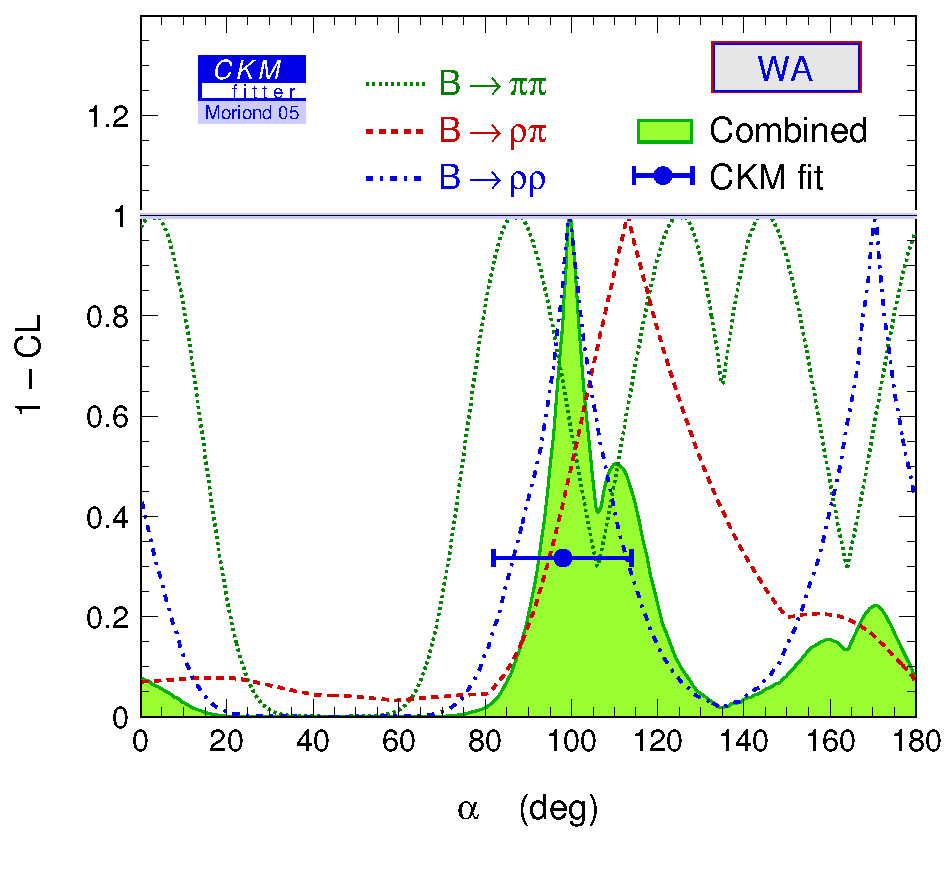
\includegraphics[width=\largefigwidth]{ckmfitter-alpha-combined}
%   \caption[CKM Fitter constraints on \alphaCKM.]%
%   {CKM Fitter constraints on \alphaCKM from combined \BToPiPi,
%     \BToRhoPi and \BToRhoRho decay analyses.}
%   \label{fig:CKMFitter}
% \end{figure}

\section{The \LHCb experiment}
\label{sec:LHCbInDetail}

Since both \bhadron{s} are preferentially produced in the same direction
and are forward-boosted along the beam-pipe, the detector is not required
to have full $4\pi$ solid-angle coverage. \LHCb takes advantage of this
by using a wedge-shaped single-arm detector with angular acceptance
\unit{10-300}{\mrad} in the horizontal (bending) plane~\cite{Amato:1998xt}.

\vspace{1cm}

\begin{center}
{\hspace{1mm}\Large\vdots\hspace{1cm}}
\end{center}

\vspace{1cm}

The detector is illustrated in \FigureRef{fig:LHCbCrossSection}, showing
the overall scale of the experiment and the surrounding cavern structure.

\begin{sidewaysfigure}
  \begin{center}
  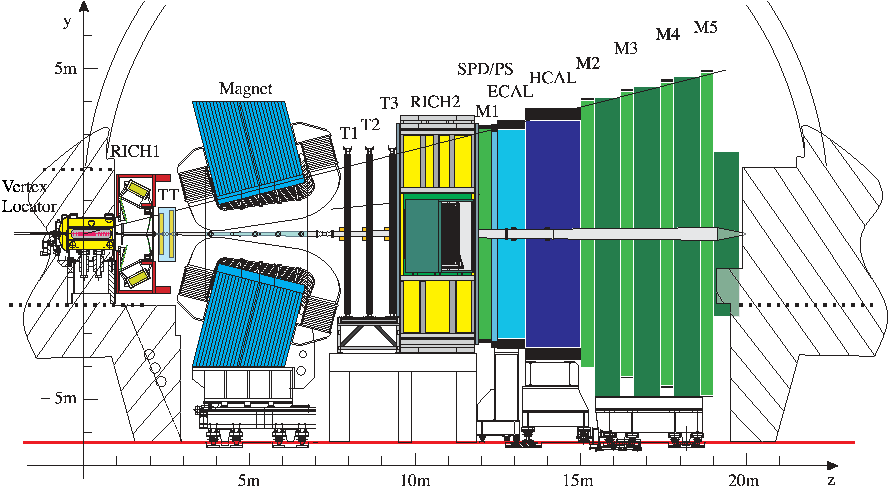
\includegraphics[width=0.8\textheight]{lhcb-detector-cross-section}
  \caption[Cross-section view of \LHCb, cut in the non-bending $y$--$z$ plane]%
    {Cross-section view of \LHCb, cut in the non-bending $y$--$z$ plane.}
  \label{fig:LHCbCrossSection}
  \end{center}
\end{sidewaysfigure}

The single-sided detector design was chosen in preference to a two-armed
design since the detector dimensions are restricted by the layout of the
IP8 (ex-Delphi) cavern in which \LHCb is located. Using all the available
space for a single-arm spectrometer more than compensates in performance
for the \about{50\percent} drop in luminosity.

\section{The \Cerenkov mechanism}
A Huygens construction in terms of spherical shells of probability for photon
emission as the particle progresses along its track shows an effective
``shock-front'' of \Cerenkov emission. This corresponds to an emission cone of
opening angle \thetaCerenkov around the momentum vector for each point on the
track,
%
\begin{subequations}
  \label{eq:cosThetaCk}
  \begin{equation}
    \cos\,\thetaCerenkov  &= \frac{1}{n \beta} +
                             \frac{\hbar k}{2p}%
                             \parenths{ 1 - \frac{1}{n^2} } \\
                          &\,\sim \frac{1}{n \beta}%
    \label{eq:cosThetaCkApprox}
  \end{equation}
\end{subequations}
%
where $\beta \equiv v/c$, the relativistic velocity fraction.

\section{Trigger system}
\label{sec:triggers}
An overview of the \LHCb trigger characteristics broken down by level
is shown in \Table~\ref{tab:TriggerDetails}.

\begin{table}[bp]
  \begin{tabular}{lllll}
                & L0              & L1              & HLT             \\
    \midrule\\
    Input rate  & \unit{40}{\MHz} & \unit{1}{\MHz}  & \unit{40}{\kHz} \\
    Output rate & \unit{1}{\MHz}  & \unit{40}{\kHz} & \unit{2}{\kHz}  \\
    Location    & On detector     & Counting room   & Counting room   \\
  \end{tabular}
  \caption{Characteristics of the trigger levels and offline analysis.}
  \label{tab:TriggerDetails}
\end{table}

    \chapter{Continued captions}
\label{chap:ContCaptions}

Here are some funky floats using ``continued captions'', i.e. for a semantically
collected group of float contents which are too numerous to fit into a single
float, such as the pretty circles in the following figure:

\newcommand{\circleimg}[1]{%
\begin{tikzpicture}
  \draw[color=black,fill=#1,thick] (1,0) circle (1.5cm);
\end{tikzpicture}%
}

\begin{figure}[hb]
  \subfloat[][Example 1a]{\label{fig:cc1a}\circleimg{red!80}}\quad
  \subfloat[][Example 1b]{\label{fig:cc1b}\circleimg{green!70!yellow}}\quad
  \subfloat[][Example 1c]{\label{fig:cc1c}\circleimg{blue!80}}\quad
  \subfloat[][Example 1d]{\label{fig:cc1d}\circleimg{orange!80!yellow}}
  \caption{Demonstration of \texttt{subfig} continued captions.}
  \label{fig:cc1}
\end{figure}

\begin{figure}[p]
  \ContinuedFloat
  \subfloat[][Example 1e]{\label{fig:cc1e}\circleimg{violet}}\quad
  \subfloat[][Example 1f]{\label{fig:cc1f}\circleimg{cyan}}\quad
  \subfloat[][Example 1g]{\label{fig:cc1g}\circleimg{magenta}}\quad
  \subfloat[][Example 1h]{\label{fig:cc1h}\circleimg{yellow}}
  \caption[]{Demonstration of \texttt{subfig} continued captions (continued).}
\end{figure}

\noindent
This mechanism means that the same float label is used for both pages of
floats. Note that we can refer to \FigureRef{fig:cc1} in general, or to
\FigureRef{fig:cc1g} on \PageRef{fig:cc1g} in particular!

\noindent
Just for the hell of it, let's also refer to \SectionRef{sec:neutralmixing}.

    \include{chap4}
 
    % bibliography
    %
    \bibliographystyle{plain}
    \bibliography{thesis}
 
    % appendices
    %
    \appendix
    \include{appxa}
    \include{appxb}
 
    \NeedsTeXFormat{LaTeX2e}
\ProvidesClass{vita}[1996/10/09
                     class file ``vita'' to create Curriculum Vitae]
%%%%%%%%%%%%%%%%%%%%%%%%%%%%%%%%%%%%%%%%%%%%%%%%%%%%%%%%%%%%%%%%%%%%%%%
%%
%% (C) Copyright 1995, Andrej Brodnik, ABrodnik@UWaterloo.CA. All
%% rights reserved.
%%
%% This is a generated file. Permission is granted to to customize the 
%% declarations in this file to serve the needs of your installation. 
%% However, no permission is granted to distribute a modified version of 
%% this file under its original name. 
%% 
%% \CharacterTable
%%  {Upper-case    \A\B\C\D\E\F\G\H\I\J\K\L\M\N\O\P\Q\R\S\T\U\V\W\X\Y\Z
%%   Lower-case    \a\b\c\d\e\f\g\h\i\j\k\l\m\n\o\p\q\r\s\t\u\v\w\x\y\z
%%   Digits        \0\1\2\3\4\5\6\7\8\9
%%   Exclamation   \!     Double quote  \"     Hash (number) \#
%%   Dollar        \$     Percent       \%     Ampersand     \&
%%   Acute accent  \'     Left paren    \(     Right paren   \)
%%   Asterisk      \*     Plus          \+     Comma         \,
%%   Minus         \-     Point         \.     Solidus       \/
%%   Colon         \:     Semicolon     \;     Less than     \<
%%   Equals        \=     Greater than  \>     Question mark \?
%%   Commercial at \@     Left bracket  \[     Backslash     \\
%%   Right bracket \]     Circumflex    \^     Underscore    \_
%%   Grave accent  \`     Left brace    \{     Vertical bar  \|
%%   Right brace   \}     Tilde         \~}
%%
%%---

%%%%%%%%%%%%%%%%%%%%%%%%%%%%%%%%%%%%%%%%%%%%%%%%%%%%%%%%%%%%%%%%%%%%%%%
%
%    - based on vita.sty by kcb@hss.caltech.edu
%    - 1995/02/07: the first version
%    - 1996/10/09: if there is no business address the field is
%                  left out
%
% User documentation: This class file only provides basic definitions
% =================== of environments, which are then used in class
% option files to instantiate entries for different disciplines. Thus,
% create your document as follows:
%
%    \documentclass[<discipline>]{vita}
%    \begin{document}
%      \name{Andrej Brodnik}
%      \businessAddress{First line \\ second line of bussines address}
%      \homeAddress{Again \\ multiline address \\ perhaps with phone number}
%    \begin{vita}
%      % here comes a real Curriculum Vitae for particular <discipline>
%    \end{vita}
%    \end{document}
%
% where it is assumed that file ``vita<discipline>.clo'' exists and defines
% proper categories used in given discipline. For detail explanation on
% categories in different disciplines see individual ``.clo'' files.
%
% The output will have format:
%
%   o on the first page will appear a title ``Curriculum Vitae'' (to
%     change it, see below under i18n notes -- internationalization)
%   o below will be your name
%   o below, side by side, your business and home address headed
%     by strings ``Business address'' and ``Home address''
%     respectively (to change these strings see below in i18n notes).
%   o then will follow the rest of CV as defined by ``<discipline>.clo''
%     file.
%   o the header of each but first page will include your name and the
%     page number.
%   o on the last page in the bottom right you will have the current
%     date, that is month and year (to change this, see below under
%     i18n notes).
%
%------
%
% i18n NOTES: If you are making CV for some other language, you have to
% =========== redefine:
%   - title:
%       o use command:   ``\title{<new title>}''
%       o default value: ``Curriculum Vitae''
%   - date:   
%       o use command:   ``\today{<date})''
%       o default value: ``<current month>, <current year>'' (in English)
%   - addresses headers:
%       o use command:   ``\HeaderBusiness{<new header>}''
%                        ``\HeaderHome{<new header>}''
%       o default value: ``Business address''
%                        ``Home address''
%
%------
%
% System documentation: class ``vita'' is based on the class
% ===================== ``article''. It changes the title into
% <default value> (see i18n notes) and the name becomes an
% author. Individual categories, publications and references are
% implemented using ``description'' environment. 
%
%----------------------------------------

%%%%
%
% Process options and load class article:
%---
\let\@optionsToInput=\@empty
\DeclareOption*{
  \IfFileExists{vita\CurrentOption.clo}%
    {\edef\@optionToInput{vita\CurrentOption.clo}}%
    {\PassOptionsToClass{\CurrentOption}{article}}
}
\ProcessOptions
\LoadClass{article}

%%%%
%
% First all i18n definitions:
%---
\title{Curriculum Vitae}
\renewcommand{\today}{
  \ifcase\month\or
    January\or February\or March\or April\or May\or June\or
    July\or August\or September\or October\or November\or December\fi,
  \space\number\year}
\newcommand\HeaderBusiness[1]{\def\@businessAddressHeader{#1}}
  \HeaderBusiness{Business Address}
\newcommand\HeaderHome[1]{\def\@homeAddressHeader{#1}}
  \HeaderHome{Home Address}

%%%%
%
% Next, header definitions:
%---
\date{\relax}
\newcommand{\name}[1]{
  \renewcommand{\@author}{#1} \markright{\protect\small\@author}
}
\newcommand{\businessAddress}[1]{\def\@businessAddress{#1}}
  \businessAddress{}
\newcommand{\homeAddress}[1]{\def\@homeAddress{#1}}
  \homeAddress{}

%%%%
%
% \maketitle command, which prints out the title and the name of person
%---
\renewcommand{\maketitle}{\newpage
  \global\@topnum\z@   % Prevents figures from going at top of page.
  \begin{center}
    {\LARGE \@title}

    \medskip

    {\large \@author}
  \end{center}

  \bigskip

  \thispagestyle{plain}

  \gdef\@author{}\gdef\@title{}
}

%%%%
%
% ``vita'' environment:
%---
\pagestyle{empty}
\newenvironment{vita}{
     % first page is empty style though the following pages have on the
     % right side written the name from the \name command
  \ifx\@author\@empty\@warning{Missing name command}\fi
     % next we start to layout information. First the title and the
     % name,

  \maketitle
     % followed by both addresses,
  \begin{tabular*}{\textwidth}{@{\extracolsep{\fill}}ll@{}}
    \begin{tabular}[t]{@{}l@{}}
    \ifx\@businessAddress\@empty\mbox{}\else
       {\small \@businessAddressHeader:}
    \\ \@businessAddress
    \fi
    \end{tabular}
  &
    \ifx\@homeAddress\@empty\@warning{Missing home address}%
    \else
      \begin{tabular}[t]{@{}l@{}}
         {\small \@homeAddressHeader:}
      \\ \@homeAddress
      \end{tabular}
    \fi
  \end{tabular*}

  \bigskip

  \thispagestyle{empty}
}{   % quite at the bottom of last page we have a date
  \par\nopagebreak\vfill\hfill \today
}%end vita environment

%%%%
%
% Curriculum vitae consists of categories which we create using
% command:
%
%      \newcategory[The name]{The label}
%
% where <The name> is written in bold character as a small title of
% category. It appears at the left margine of a page. If <The name>
% parameter is missing, it takes the same value as <The label>, which,
% in turn is used to refer to individual category. For example
% commands:
%
%      \newcategory{Name of category}
%      \newcategory[Name of category]{Name of category}
%
% have the same result. Now, to use category:
%
%      \newcategory[Some category]{some other name}
%
% the input has form:
%
% \begin{some other name}
%   \item The first item
%   \item The second one etc.
% \end{some other name}
%
% and the category will have on the output title ``Some category''.
% Entries in each category are preceded by \item.
%
%-----
% i18n NOTE: One can use as the names of categories strings in
% ========== different languages, but the labels can be the same in
% the same language, which is useful if you have a single CV and you
% want outputs in different languages.
%---
\def\@newCategory[#1]#2{%
  \newenvironment{#2}{\medskip\pagebreak[2]\par
    \textbf{\small #1}\nopagebreak
    \begin{description}}{\end{description}\par}
}
\def\@noNameCategory#1{\@newCategory[#1]{#1}}
\def\newcategory{\@ifnextchar[{\@newCategory}{\@noNameCategory}}

%%%%
%
% Inside categories we have different ``kinds'' (such as different
% publications), which we create using command \newkind. It has the
% same parameters as \newcategory and all comments at command
% newcategory are also valid here.
%---
\def\@newKind[#1]#2{%
  \newenvironment{#2}{
    \pagebreak[2]
    \item \textbf{\small #1}\nopagebreak
      \begin{description}
  }{  \end{description}\par }
}
\def\@noNameKind#1{\@newKind[#1]{#1}}
\def\newkind{\@ifnextchar[{\@newKind}{\@noNameKind}}

%%%%
%
% There is a special category ``plaincategory'' which entries are
% simply listed without any indentation, and in particular, multiple
% references are separated by \and command. It can be used for
% references.
%---
\def\@newPlainCategory[#1]#2{%
  \newenvironment{#2}{
    \medskip\pagebreak[2]\par
    \textbf{\small #1}\nopagebreak
    \renewcommand{\and}{
             \end{tabular}
      \item[]\begin{tabular}[t]{l}
    }
    \begin{description}
    \item[] \begin{tabular}[t]{l}
  }{        \end{tabular}
    \end{description}\par
  }
}
\def\@noNamePlainCategory#1{\@newPlainCategory[#1]{#1}}
\def\newplaincategory{\@ifnextchar[{\@newPlainCategory}{\@noNamePlainCategory}}

%%%%
%
% Finally, formatting parameters and the possible option to input:
%---
\pagestyle{myheadings}
\parindent 0pt
\nofiles

\ifx\@optionToInput\@empty\relax
\else \input \@optionToInput
\fi
 
    \end{document}
  \end{verbatim}
 \end{fullpage}
\end{figure}
 
The first section, from the \verb"\documentclass" to
the \verb"\begin\{document\}", defines the document class and options.
This thesis has specified two-sided formatting, which is now
allowed by the Graduate School.  Two sided printing is now
actually \LaTeX's default.  If you want one sided printing
you must specify \verb"oneside".
This sample also specified a font size
of 11 points. 
Possible font size options are: \verb"10pt", \verb"11pt", and \verb"12pt".
Default is 12 points, which is the preference
of the Graduate School. If you choose a smaller size be sure to
check with the Graduate School for acceptability.  The smaller fonts
can produce very small sub and superscripts.

Include most additional formatting packages with \verb"\usepackage",
as describe by Lamport\cite{Lbook}.  The one exception to this
rule is the \verb"natbib" package.  Include it with the \verb"natbib"
document option.
 
Use the \verb"\includeonly" command to format only a part of your
thesis.  See Lamport\cite[sec. 4.4]{Lbook} for usage and limitations.

 
\section{The Text Pages}
 
A chapter is a major division of the thesis.  Each chapter begins
on a new page and has a Table of Contents entry.
 
\subsection{Chapters, Sections, Subsections, and Appendices}
 
 
Within the chapter title use a \verb"\\" control sequence to separate lines
in the printed title (recall Figure \ref{start-2}.).
The \verb"\\" does not affect the Table of Contents entry.
 
Format appendices just like chapters.
The control sequence \verb"\appendix" instructs \LaTeX\ to
begin using the term `Appendix' rather than `Chapter'.
 
 
Sections and subsections of a chapter are specified
by  \verb"\section" and \verb"\subsection", respectively.
In this thesis chapter and section
titles are written to the table of contents.
Consult Lamport\cite[pg. 176]{Lbook} to see which
subdivisions of the thesis can be written to the table of contents.
The \verb"\\" control sequence is not permitted in section and
subsection titles.
 
 
\subsection{Footnotes}
 
\label{footnotes}
 Footnotes format as described in the \LaTeX\ book.  You can also
 ask for end-of-chapter or end-of-thesis notes.
 The thesis class will automatically set these up if
 you ask for the document class option \texttt{chapternotes}
 or \texttt{endnotes}.  
 
If selected, chapternotes will print automatically.  If you choose
endnotes however you must explicitly indicate when to print the notes 
with the command \verb"\printendnotes".  See the style guide for
suitable endnote placement.  

\subsection{Figures and Tables}
Standard \LaTeX\ figures and tables, see Lamport\cite[sec.~C.9]{Lbook},
normally provide the most convenient means to position the figure.
Full page floats and facing captions are exceptions to this rule.

If you want a figure or table to occupy a full page enclose the
contents in a \texttt{fullpage} environment.  
See figures~\ref{facing-caption}.

Facing page captions are described
in the Style Manual\cite{SP}.  They have different meanings
depending on whether you are using
the one-side or two-side thesis style.


If you are using the two-side style,
facing captions
are full page captions for full page figures or tables
and must face the illustration to which they refer.
You must explicitly format both pages. 
The caption part must appear on an even page
(left side) and the figure or table must
come on the following odd page (right side).
Enclose the float contents for the caption 
in a \texttt{leftfullpage} environment,
and enclose the float contents for the figure or table 
in a \texttt{fullpage} environment.
Figure~\ref{control-file}, for example,
required a full page so its caption (on a facing caption page)
would have been formatted as shown in figure~\ref{facing-caption}a.
The first page (left side) contains the caption. The second page
(right side) could be left blank.  A picture or graph might be pasted onto
this space.


\begin{figure}[t]
\footnotesize
\begin{verbatim}
     \begin{figure}[p]% the left side caption
       \begin{leftfullpage}
         \caption{ . . . }
       \end{leftfullpage}
     \end{figure}
     \begin{figure}[p]% the right side space
       \begin{fullpage}
          . . .
          ( note.. no caption here )
       \end{fullpage}
     \end{figure}
\end{verbatim}
\caption(a){This text would create a
  double page figure in the two-side style.}
\label{facing-caption}
\end{figure}
 
\begin{figure}[t]
\footnotesize
\begin{verbatim}
     \begin{figure}[p]
        \begin{leftfullpage}
           \caption{ . . . }
        \end{leftfullpage}
     \end{figure}
     \begin{figure}[p]% the right side space
       \begin{xtrafullpage}
          . . .
          ( note.. no caption here )
       \end{xtrafullpage}
     \end{figure}
\end{verbatim}
\caption(b)[Generating a facing caption page]{This text would create a
  facing caption page with the accompaning figure in the one-side style.}
\end{figure}
 
If instead you are using the one-side style,
facing caption pages are still
captions for full page figures or tables
that appear on the left-hand page (facing the illustration on the
right-hand page).  
However, the page number and binding offset are reversed
from their normal positions.
Format these captions by enclosing the float contents
in a \texttt{leftfullpage} environment.
Because you are printing on only one side of each sheet, you must manually
turn over this caption sheet. 
You then have the choice of inserting a preprinted illustration or
formatting one to print with the thesis. 
In either case no page number should appear
on the illustration page, nor should the page number increment. 
Enclose your figure's text
in an \texttt{xtrafullpage} environment, which will cause the
page numbers to come out right.  
You can, of course, leave out the illustration and insert a preprinted
copy later. 
Figure~\ref{facing-caption}b shows how to format a facing caption page
in the one-side style. Note that, in this case, the illustration
was also printed.

In the two-side style the \texttt{xtrafullpage} environment acts just like the
\texttt{fullpage} environment.  It does not produce a numberless page.


 
\subsection{Horizontal Figures and Tables}
Figures and tables may be formatted horizontally
(a.k.a.\ landscape) as long as their captions appear
horizontal also.  \LaTeX\ will format landscape material for you
if a couple of conditions are met.  You have to have a printer
and printer driver that allow rotations and
you have to have a couple of add-on \LaTeX\ packages.  

% Users of PostScript printers and Uniform Access computers 
% at the University of Washington will conform to both requirements,
% as will users of PC\TeX\ if they use postscript.

Include the \texttt{rotating} package 
\begin{demo}
\\usepackage[figuresright]\{rotating\}
\end{demo}
and read the documentation that comes with the package. 

Figure~\ref{sideways} is an example of how a landscape
table might be formatted. 

\begin{figure}[t]
\footnotesize
\begin{verbatim}
     \begin{sidewaystable}
         ...
         \caption{ . . . }
     \end{sidewaystable}
\end{verbatim}
\caption[Generating a landscape table]{This text would create a
  landscape table with caption.}
\label{sideways}
\end{figure}
 


\subsection{Figure and Table Captions}
Most captions are formatted with the \verb"\caption" macro as described 
by Lamport\cite[sec. C.9]{Lbook}. 
The uwthesis class extends this macro to allow
continued figures and tables, and to provide multiple figures and
tables with the same number, e.g., 3.1a, 3.1b, etc.
 
To format the caption for the first part of
a figure or table that cannot fit
onto a single page use the standard form:
\begin{demo}
\\caption[\textit{toc}]\{\textit{text}\}
\end{demo}
To format the caption for the subsequent parts of 
the figure or table 
use this caption:
\begin{demo}
\\caption(-)\{(continued)\}
\end{demo}
It will keep the same number and the text of the caption will be 
{\em(continued)}.

To format the caption for the first part of
a multi-part figure or table
use the format:
\begin{demo}
\\caption(a)[\textit{toc}]\{\textit{text}\}
\end{demo}
The figure or table will be lettered (with `a') as well as numbered.
To format the caption for the subsequent parts of 
the multi-part figure or table
use the format:
\begin{demo}
\\caption(\textit{x})\{\textit{text}\}
\end{demo}
where {\em x} is {\tt b}, {\tt c}, \ldots.
The parts will be lettered (with `b', `c', \ldots).

\section{The Preliminary Pages}
 
These are easy to format only because they are relatively invariant
among theses.  Therefore the difficulties have already been encountered
and overcome by \LaTeX\ and the thesis document classes.
 
\subsection{Title page}
Define \verb"\Title", \verb"\Author", \verb"\Program", and \verb"\Year" 
and then print the
title page with \verb"\titlepage".
The title page of this thesis was printed with%
\footnote{Actually, it wasn't.  It included a footnote---unusual for
  title pages.}
 
\begin{demo}
\\Title\{The Suitability of the \\LaTeX\\ Text Formatter\\\\
   for Thesis Preparation by Technical and\\\\
   Non-technical Degree Candidates\}
\\Author\{Jim Fox\}
\\Program\{UW Technology Services\}
\\Year\{1999\}
\\titlepage
\end{demo}
 
You may also change other text on the  title page with these
macros.  You will have to redefine \verb"\Degreetext", for instance,
if you're writing a Master's thesis instead of a dissertation.

\begin{list}{}{\itemindent\parindent\itemsep0pt
   \def\makelabel#1{\texttt{\char`\\#1}\hfill}}
\item[Degree\char`\{{\it degree name}\char`\}]
   defaults to ``Doctor of Philosophy''
\item[School\char`\{{\it school name}\char`\}] defaults to
``University of Washington''
\item[Degreetext\char`\{{\it degree text}\char`\}] defaults to
``A dissertation submitted \ldots''
\end{list}

These definitions must appear \underline{before} the \verb"\titlepage" command.

\subsection{Signature page}
Define \verb"\Chair" and as many \verb"\Signature" lines as
you need
and then print the
signature page with \verb"\signaturepage".
The signature page of this thesis was printed with
 
\begin{demo}
\\Chair\{Name of Chairperson\}\{title\}\{Chair's department\}

\\Signature\{Name of Committee member\}
\\Signature\{Name of Committee member\}
\\Signature\{etc\}
\\signaturepage
\end{demo}
 
You have to put in the real names.  Notice the definition
of \verb"\Chair" has three arguments. 
The second (Chair's title) and third (Chair's department)
will be used on the Abstract page.

If you have co-chairs just repeat the \verb"\Chair" definition.

For a Master's Thesis omit the \verb"\Chair" definitions and
use \verb"\thesissignaturepage".

\subsection{Quote slip}
Use one of the ``quoteslip'' macros to format your quote slip:

\begin{itemize}
\item \verb"\thesisquoteslip", for a master's thesis;
\item \verb"\doctoralquoteslip", for a doctoral dissertation; or
\item \verb"\doctoralabstractquoteslip", for a the `abstract only' 
form of the doctoral dissertation.
\end{itemize}

\noindent
None of these macros takes an argument.  They use the
text suggested by the Graduate School\cite{SP}. 

If you need nonstandard quote slip text
use the \verb"\quoteslip" macro instead.
It has one argument, which is the text of your quote slip.
The quote slip of this thesis was printed with
\begin{demo}
\\quoteslip\{Extensive copying . . . may be found.\}
\end{demo}
 
\subsection{Abstract}
Print the
abstract with \verb"\abstract".
It has one argument, which is the text of the abstract.
All the names have already been defined.
The abstract of this thesis was printed with
 
\begin{demo}
\\abstract\{This sample . . . `real' dissertation.\}
\end{demo}
 
 
\subsection{Tables of contents}
Use the standard \LaTeX\ commands to format these items.
 
 
\subsection{Acknowledgments}
Use the \verb"\acknowledgments" macro to format the acknowledgments page.
It has one argument, which is the text of the acknowledgment.
The acknowledgments of this thesis was printed with
 
\begin{demo}
\\acknowledgments\{The author wishes . . . \{\\it il miglior fabbro\}.\\par\}\}
\end{demo}
 
 
\subsection{Dedication}
Use the \verb"\dedication" macro to format the dedication page.
It has one argument, which is the text of the dedication.
 
\subsection{Vita}
Use the \verb"\vita" macro to format the curriculum vitae.
It has one argument, which chronicles your life's accomplishments.

Note that the Vita is not really a preliminary page.
It appears at the end of your thesis, just after the appendices.
 
 
%%  
%% \section{Customization of the Macros}
%%  
%% Simple customization, including 
%% alteration of default parameters,  changes to dimensions,
%% paragraph indentation, and margins, are not too difficult.
%% You have the choice of modifying the class file ({\tt uwthesis.cls})
%% or loading
%% one or more personal style files to customize your thesis.
%% The latter is usually most convenient, since you do not need
%% to edit the large and complicated class file.
%% 
 


% ========== Chapter 4
 
\chapter{Hardware Dependencies\\
  ({\it And Other Complications})}
 
 
\TeX\ has been designed to produce exactly the same document
on all computers and on all printers.  {\it Exactly the same}
means that the various spacings, line and page breaks, and
even hyphenations will occur at the same places
when the document is formatted on a variety of computers.
However, there are some discrepancies that cannot
be overcome.  They involve the mechanics of running \TeX\ and
the necessary variations in computer and
output device capability.
 
\section{Running \protect\LaTeX}
 
Each operating system has some means for editing and storing text,
starting programs, and printing program output.  These
are uniformly inconsistant between machines.  Therefore there
are no useful, generic instructions for running \LaTeX.
You will have to
be able to do the following on your chosen computer.
 
\begin{itemize}
\item Create, edit, and back-up text files.
\item Run the \TeX\ program with \LaTeX\ format.
\item Convert the device independent output
  to a format suitable to the selected printer.
\item Print the converted file.
\end{itemize}
 
There are generally user's manuals available for each \TeX\
implementation, which explain the program's local procedures
and nuances.
 
\section{Fonts}
 
Different printers, and different sites with identical
printers, make certain sets of fonts available for their users.
While these font sets are not identical, they do have a common
subset---the basic roman fonts.
Most sites will also provide fonts at standard magnifications
(\verb"\small", \verb"\large", \verb"\Large", etc.).
The Graduate School wants a larger type than is normally used
for book printing.  The uwthesis document class uses 11-point.

The postscript font New Century Schoolbook also prints a nice thesis.
Request it with:
\begin{demo}
\\usepackage\{newcent\}
\end{demo}
 
 
\section{Printer Perversity}
 
\begin{flushright}
  \footnotesize \it
  Never let anything mechanical know you are depending on it.
\end{flushright}
 
\medskip
 
A printer will break the day before a dissertation is due.  This is
an immutable law of nature.  Print your dissertation well in advance
of any deadlines.  Take some time to admire your work.
 


\printendnotes

%
% ==========   Bibliography
%
\nocite{*}   % include everything in the uwthesis.bib file
\bibliographystyle{plain}
\bibliography{uwthesis}
%
% ==========   Appendices
%
\appendix
\raggedbottom\sloppy
 
% ========== Appendix A
 
\chapter{Where to find the files}
 
The uwthesis class file, {\tt uwthesis.cls}, contains the parameter settings,
macro definitions, and other \TeX nical commands which
allow \LaTeX\ to format a thesis.  
The source to
the document you are reading, {\tt uwthesis.tex},
contains many formatting examples
which you may find useful.
The bibliography database, {\tt uwthesis.bib}, contains instructions
to BibTeX to create and format the bibliography.
You can find the latest of these files in the following locations:

\begin{itemize}
\item CTAN
\begin{description}
\item[]  \verb%http://tug.ctan.org/tex-archive/macros/latex/contrib/uwthesis/%
\end{description}

\item My page.
\begin{description}
\item[] \verb%http://staff.washington.edu/fox/tex/uwthesis.html%
\end{description}

\end{itemize}

\vita{Jim Fox is a Senior Software Engineer at the University of Washington.
His duties do not include maintaining this package.  It is rather
an avocation which he maintains as he deems fit.

He welcomes your comments to {\tt fox@washington.edu}.
}


\end{document}
